\subsection{Or2yw Toolkit}
We use dataset $menu.csv$ from The New York Public Library, where it is a mix of simple bibliographic description of the menus (created by The New York Public Library) and the culinary and economic content of the menus themselves (transcribed by users)\cite{whatsonmenu}. We could expect how low the dataset's data quality could be that integrates manual and systematic input.

There are three modes in or2yw toolkit, including sequential, parallel and merge. Sequential mode is by directly translate the data cleaning workflow from the original JSON file (see Figure \ref{fig:recipe}), step by step without considering the dependency relationships among operations. 

Compared with Sequential mode, the parallel mode aims to recover the dependencies in the recipe on column level. Here are certain conditions that define parallel operations. 

\textbf{Parallel Node}: Operations in OpenRefine are applied row-wise and are stateless: no state is maintained among the processing of rows \cite{delpeuch2019complete}. It is thus easy to parallelize the operations if the operations are executed under different columns, as they amount to a pure map on the list of rows. Operations on different columns are expected to be mutually exclusive and not affect each other, while any actions on the same column following those parallel operations will be executed sequentially. 

\textbf{Join Node}: Two or more parallel operations will be joined together if there is one operation that combines two or more columns as input parameter in the recipe. The joined operation will be executed respectively to the latest transaction on each column preceding this operation. E.g. operation $Add column based on this column...$ allows users to concatenate multiple columns and create a new column. 

\textbf{Split Node}: One or more new nodes will be generated if an operation produces multiple columns. The new generated columns are mutually exclusive, therefore, they could be seen as parallel node.  


\begin{figure}
\centering
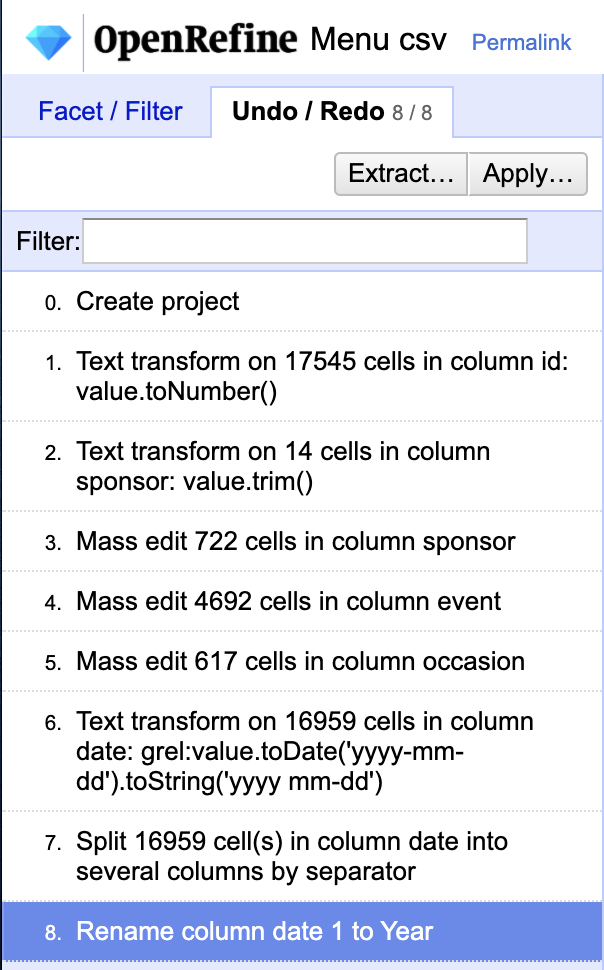
\includegraphics[width=5cm]{Figure/OR_recipe.png}
\caption{Operation History in OpenRefine}
\label{fig:recipe}
\end{figure}

\afterpage{%
\begin{figure}
  \centering
  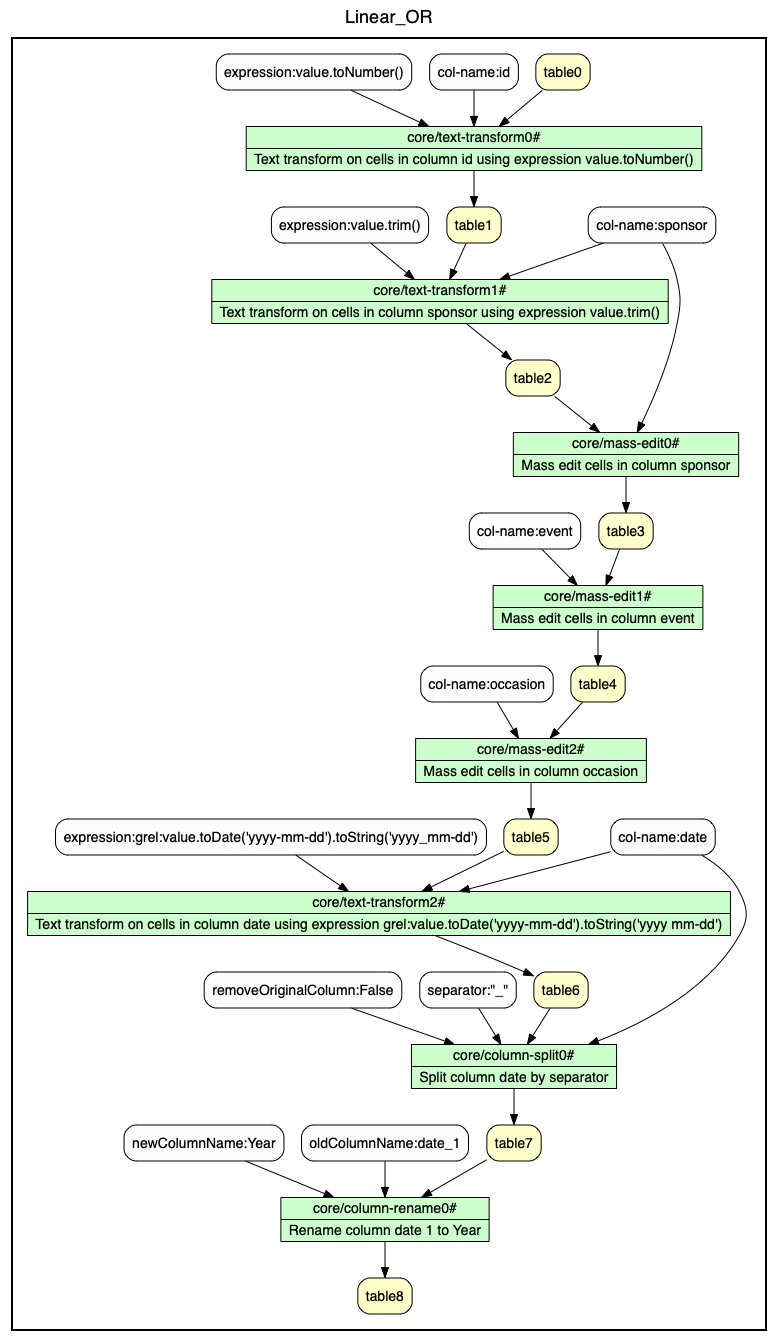
\includegraphics[width=0.7\linewidth]{Figure/dc_linear.png}
  \caption{Sequential: There are eight steps in the recipe, green box stands for the transformations, white box stands for input parameters, and yellow box represents the data stream.}
  \label{fig:sub1}
\end{figure}
\clearpage
}


\begin{landscape}

\afterpage{%
\begin{figure}
  \centering
  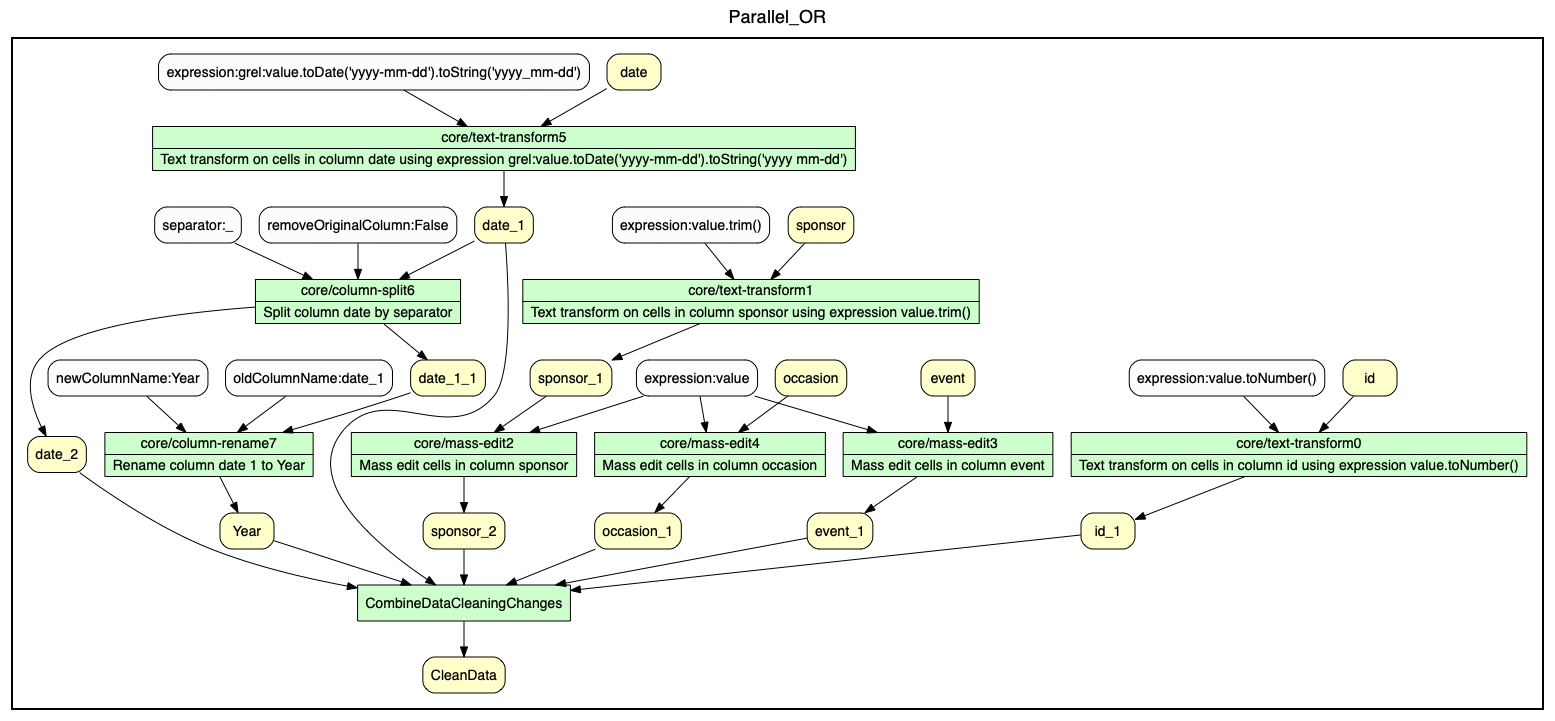
\includegraphics[width=1\linewidth, scale =1]{Figure/dc_parallel.png}
  \caption{Parallel: Transformations on column $date$, $sponsor$, $occasion$, $event$ and $id$ are parallel nodes; Split node generates by applying column-split on $date\_1$, where there are two new nodes generated, $date\_1\_1$ and $date\_2$; In the final status, $CombineDataCleaningChanges$ will merge all of the changed columns, where we could see this as Join node. }
  \label{fig:sub2}
\end{figure}
\clearpage
}
\end{landscape}


%\caption{Sequential VS Parallel: From syntactic perspective, Sequential mode is like depth-first Tree, while Parallel tends to be breadth-first tree. Parallel mode could illustrates concurrency better.}
%\label{fig:test}
%\end{figure}

%\begin{figure}

%\begin{subfigure}{.5\textwidth}
%  \centering
%  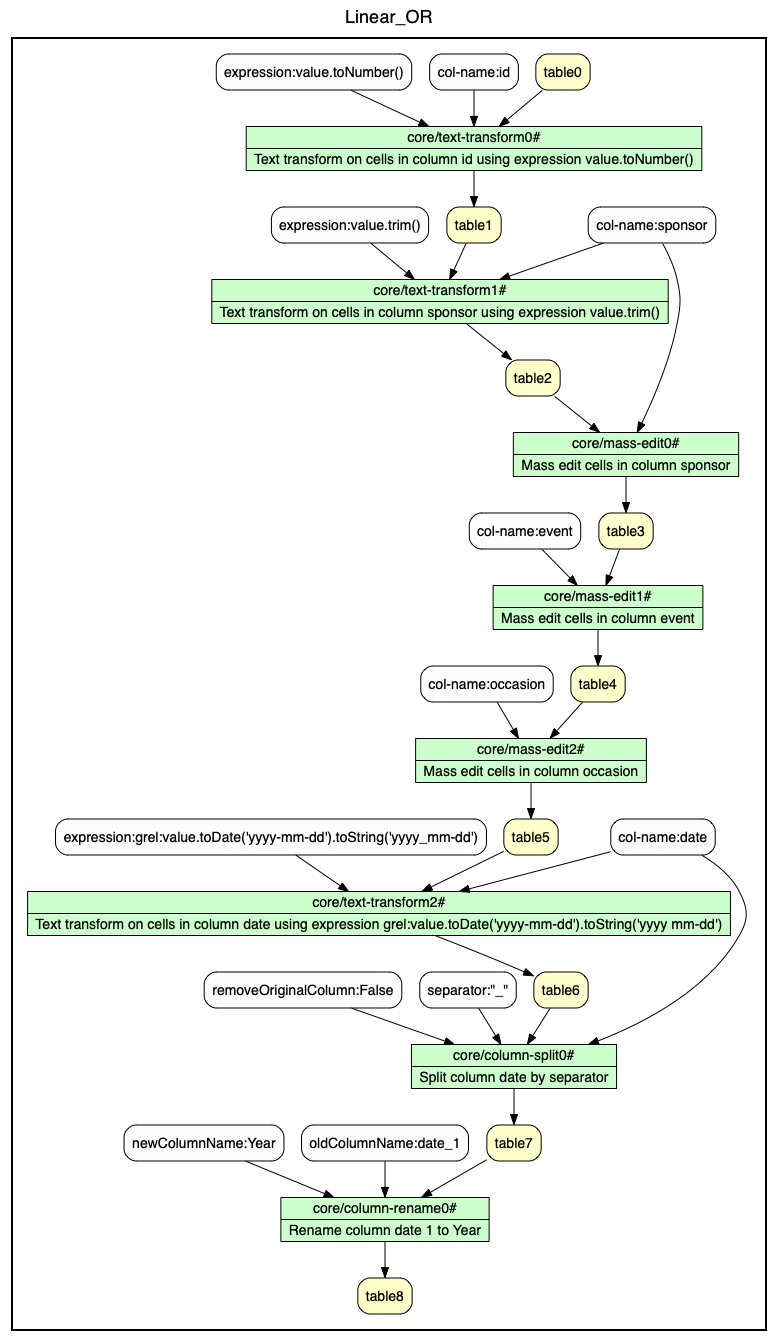
\includegraphics[width=0.6\linewidth]{Figure/dc_linear.png}
%  \caption{Sequential: There are eight steps in the recipe, green box stands for the transformations, white box %stands for input parameters, and yellow box represents the data stream.}
 % \label{fig:sub1}
%\end{subfigure}%
%\begin{subfigure}{.4\textwidth}
%  \centering
%  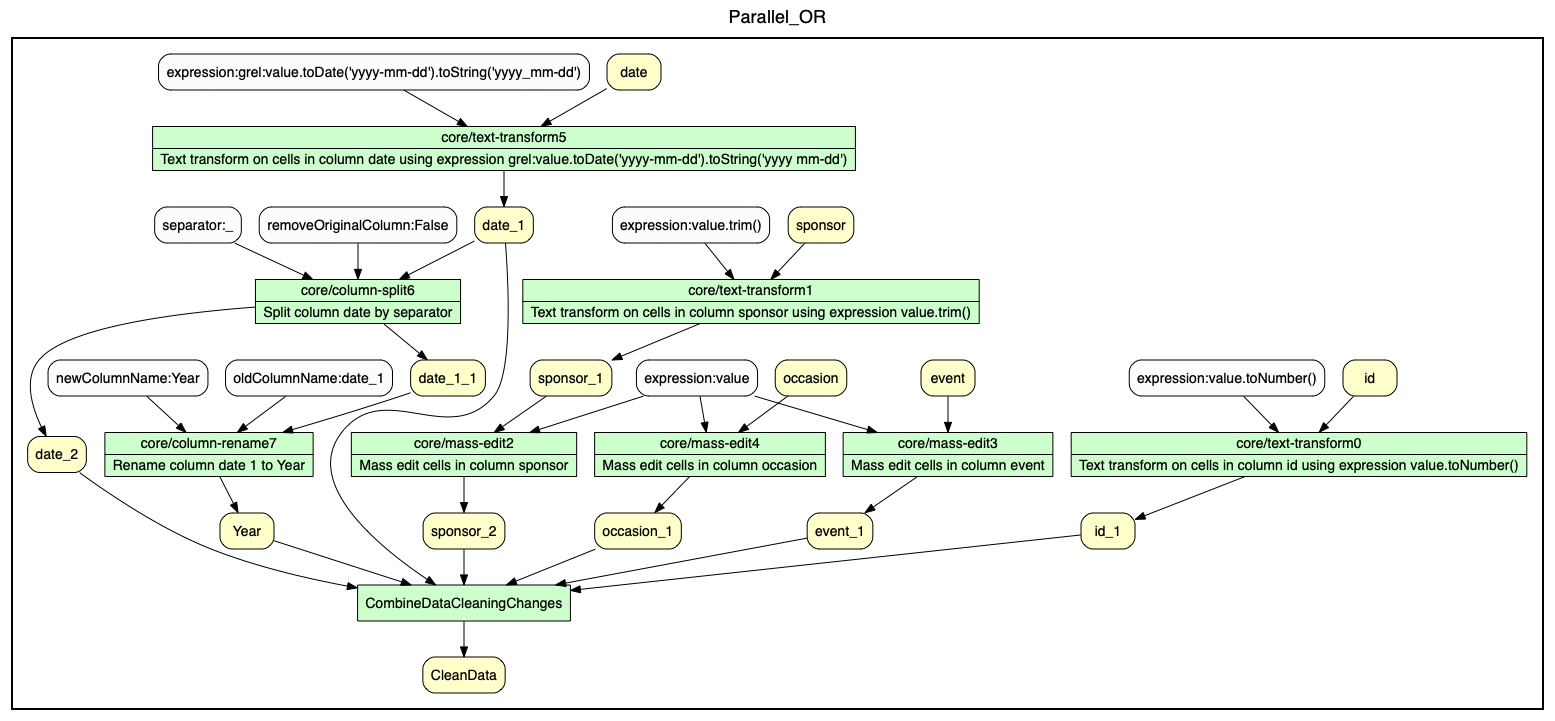
\includegraphics[width=1.6\linewidth, scale =1]{Figure/dc_parallel.png}
%  \caption{Parallel: Transformations on column $date$, $sponsor$, $occasion$, $event$ and $id$ are parallel nodes; Split node generates by applying column-split on $date\_1$, where there are two new nodes generated, $date\_1\_1$ and $date\_2$; In the final status, $CombineDataCleaningChanges$ will merge all of the changed columns, where we could see this as Join node. }
%  \label{fig:sub2}
%\end{subfigure}
%\caption{Sequential VS Parallel: From syntactic perspective, Sequential mode is like depth-first Tree, while Parallel tends to be breadth-first tree. Parallel mode could illustrates concurrency better.}
%\label{fig:test}
%\end{figure}


The merge mode is mainly dealing with recipe which is of high volume or has many "redundant" operations. Although the or2yw toolkit can produce the workflow, the output has so many nodes that it is too messy and complicated to trace. For this reason, we propose a method to merge those redundancies, where redundancy means same operations with different parameters applying on the same column. By examining the column name, or2yw toolkit will find the same operations that are executed sequentially and join them together to produce only one operation node. A separated text file is provided representing a sub-workflow that contains detailed operations and stores the parameter information as a node description. With this approach, we can produce a typical workflow for a large process with redundant operations without losing the provenance. 



\subsection{Queries with Hybrid Provenance}

Through pairing the history ID between $data.txt$ and $hisotry$ folders, we could get hybrid provenance (See Figure \ref{fig:hp process}).



\begin{figure}

\begin{subfigure}{.5\textwidth}
  \centering
  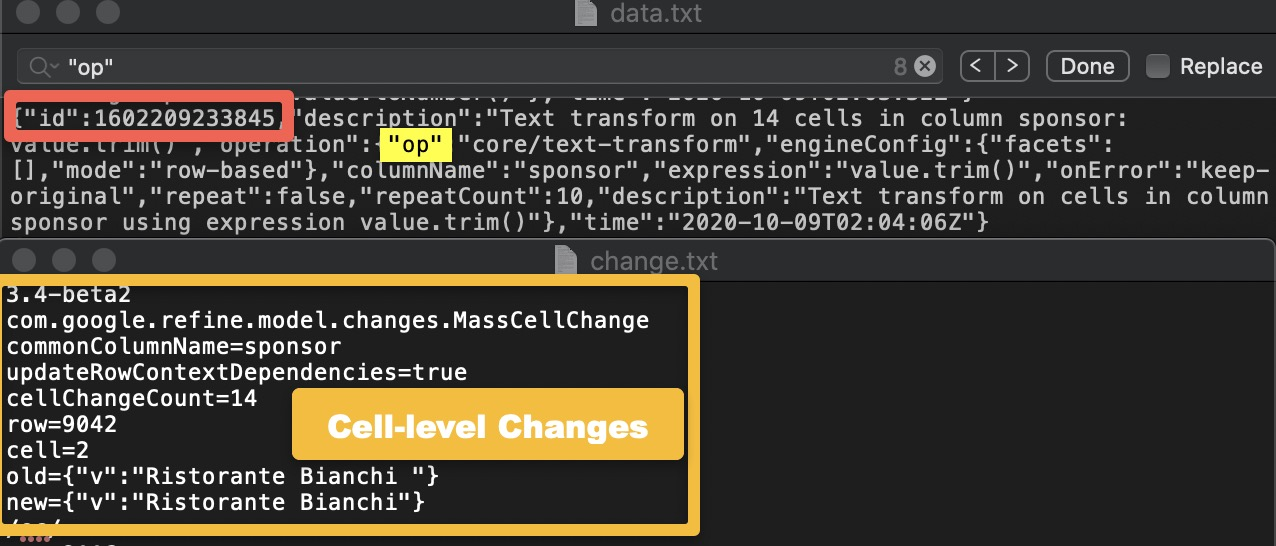
\includegraphics[width=1\linewidth, scale=1]{Figure/data-his-pair.jpeg}
  \caption{Red box is the history ID in $data.txt$, yellow box includes the cell-level changes from $history$. Provenance at cell-level would be rewritten into JSON file, and combined with changes in $data.txt$. In this way, we could get hybrid provenance (see Figure \ref{fig:hp})}
  \label{fig:pair}
\end{subfigure}%
\hspace{1em}
\begin{subfigure}{.4\textwidth}
  \centering
  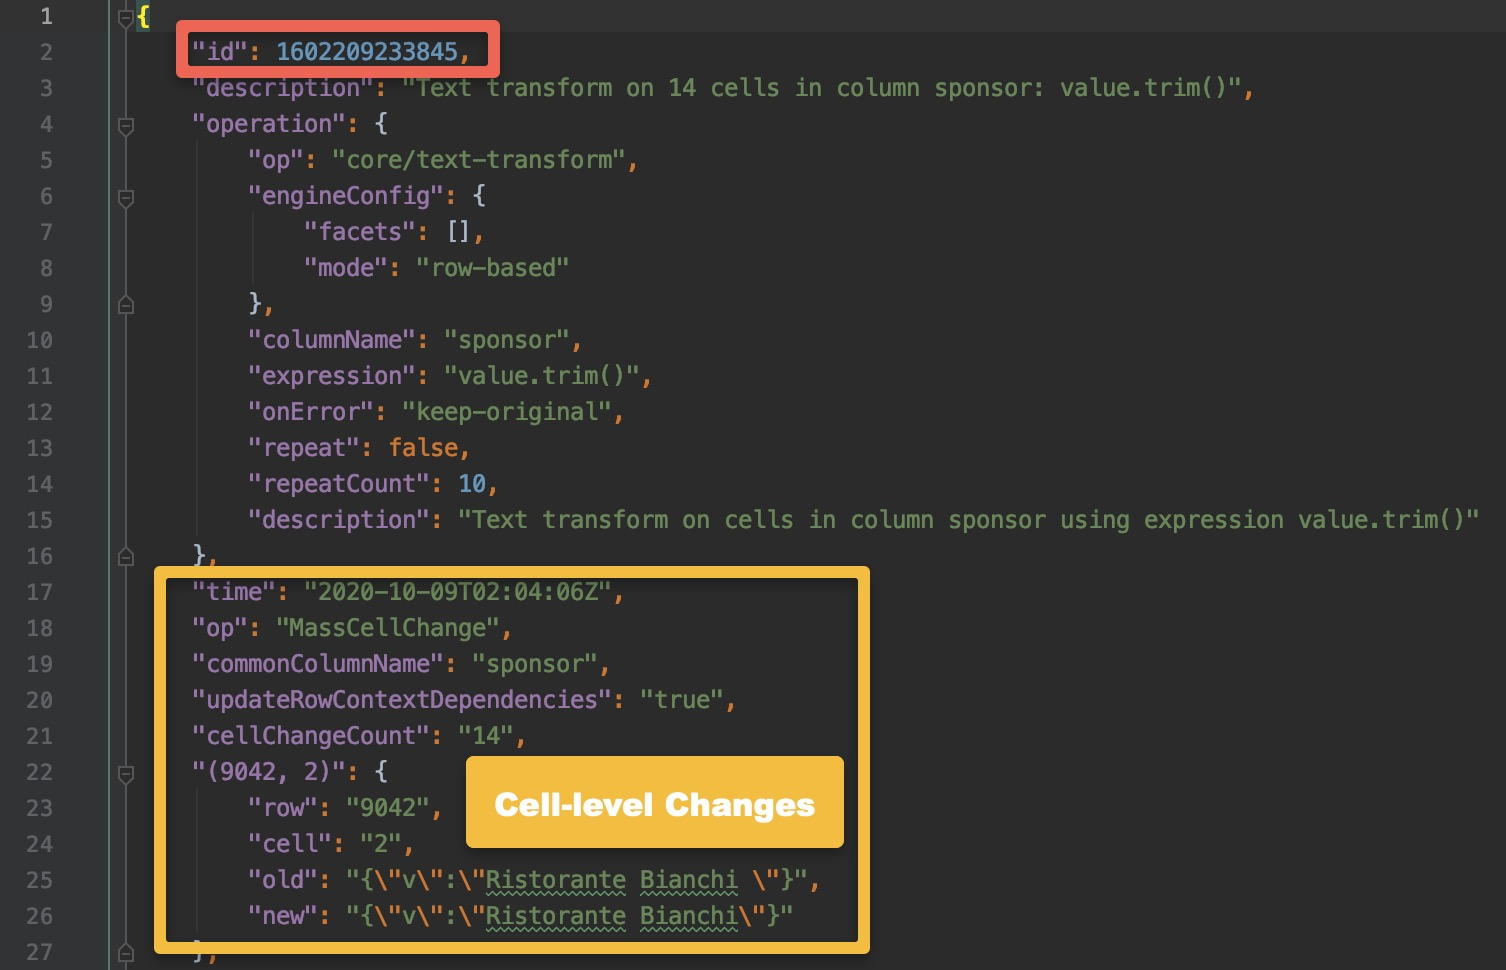
\includegraphics[width=1\linewidth, scale =0.8]{Figure/Hybrid.jpeg}
  \caption{Hybrid provenance is in JSON format, composed of provenance information in operation-level from $data.txt$ and in cell-level from $history$. }
  \label{fig:hp}
\end{subfigure}
\caption{}
\label{fig:hp process}
\end{figure}


Given the provided hybrid provenance, we would like to ask specific
questions about what its individual operation history was, how a given value in a cell came to be, reverse the data cleaning if we could get the original value. Metaphorically, we illustrate the data cleaning workflow as a collection of leaves along a flowing river: leaves are the cells in the dataset as the first-class citizens with an interesting life of their own. Many of the leaves will be lost, but for the surviving ones we are supposed to be able to tell their history as long as we know their traces in the river \cite{nunez2020first}.

In the query table (See Table \ref{tab:hybrid_prov}), there are eight queries in total. Consider given a "weird" cell value after a chain of data cleaning steps, there are some possible situations. Case one, there is no operation applied on this single cell, data quality is upstream and data is not cleaned thoroughly. Case two, an inappropriate cluster function is applied and errors are introduced. Case three, even if the value appears to be unchanged from the input, while multiple operations have been applied and the effects can be offset each other. For the previous two cases, it would be easy to trace the provenance with the help of OpenRefine recipe. Nevertheless, for the last case, the data was in fact changed during the data cleaning workflow multiple times and ended up having the same value. Fine-grained cell-level provenance information is required to inspect what really happened. Query 1,2 and 8 will return the story of a single cell. Query 3,4,6 and 7 are the quantitative analysis. Query 5 reverse the data cleaning task and return the derivation of cell value. 



\begin{table}
    \centering
    \begin{tabular}{c|c}
    \hline
    \textbf{Query Description} & \textbf{Query Command} \\
    \hline
    List all of changes applied on the given cell & changes-single-cell \\
    \hline
    List all of operations applied on the given cell & operations-single-cell \\
    \hline
    Count how many changes applied on the given cell & count-changes-single-cell \\
    \hline
    Count how many operations applied on the given cell & count-operation-single-cell \\
    \hline
    Reverse the data cleaning task and return the original cell value & reverse-data \\
    \hline
    List all of the cells indexes which get changed & list-changed-cells \\
    \hline
    Count how many cells have been changed & count-changed-cells \\
    \hline
    Provenance of the given cell & prov-single-cell \\
    \hline
    Return the answer of the whole query table & merge \\
    \hline
    \end{tabular}
    \caption{Hybrid Provenance Query table}
    \label{tab:hybrid_prov}
\end{table}


